%======================================================
% This file is part of
% "AMCOS_booklet"
% Version 1.1 (04/07/2019)
% A LaTeX template for conference books of abstracts
%
% This template is available at:
% https://github.com/maximelucas/AMCOS_booklet
%
% License: GNU General Public License v3.0
%
% Authors:
% Maxime Lucas (ml.maximelucas@gmail.com)
% Pau Clusella
%=======================================================

\documentclass[openany, parskip=full, 12pt, a4]{scrbook}

%======================================================
% This file is part of
% "AMCOS_booklet"
% Version 1.1 (04/07/2019)
% A LaTeX template for conference books of abstracts
%
% This template is available at:
% https://github.com/maximelucas/AMCOS_booklet
%
% License: GNU General Public License v3.0
%
% Authors:
% Maxime Lucas (ml.maximelucas@gmail.com)
% Pau Clusella
%=======================================================

\usepackage[utf8]{inputenc}
\usepackage[T1]{fontenc}

%---------------------------------------------------------
% PACKAGES
%---------------------------------------------------------

% TYPOGRAPHY
\usepackage{xspace}
\usepackage{microtype}
\usepackage{cmbright} % different fonts

% VARIA
\usepackage{color}
\usepackage[table, xcdraw]{xcolor} % loads also »colortbl« %load before tikz if options
\usepackage{scrhack} % fix koma script warning about addtolist
\usepackage{blindtext}
\usepackage{pdfpages} % for cover 

\usepackage{ifthen} % to have online and printed versionw

% GRAPHICS & FIGURES & TABLES
\usepackage{graphicx}
\usepackage{float}
\usepackage{multicol} % for timetable
\usepackage{multirow} % for timetable
\usepackage{longtable} % for list of participants over more than 1 page
%\usepackage{wrapfig}
%\usepackage{tikz}
%\tikzset{ar/.style={>=latex, ->}}
%\renewcommand{\arraystretch}{1.2}
%\usepackage[multidot]{grffile}
\usepackage{booktabs}
\usepackage[normalem]{ulem}                                                                        
\useunder{\uline}{\ul}{}

%BASARIM HEADER
\usepackage{fancyhdr}
\usepackage{afterpage} %To insert page number after abstract header

% WANTS TO BE LAST
\usepackage[english]{babel}

%<<<<<<< HEAD
%\usepackage[hidelinks]{hyperref}
%\hypersetup{pdfpagelayout=TwoPageRight}
%=======
\usepackage[hidelinks]{hyperref}
\hypersetup{pdfpagelayout=TwoPageRight,
            colorlinks=true,
            linkcolor=black,
            %filecolor=magenta,
            urlcolor=basarimgold}
%>>>>>>> 411df6c901ca4ee610ba56dd70ac107a3c0f62bc
% \usepackage[ocgcolorlinks]{hyperref}
% \hypersetup{colorlinks, linkcolor={wolf}, linktocpage=true, citecolor ={tpred}, urlcolor={black}}


%-------------------------------------------------------------
% SETTINGS
%-------------------------------------------------------------
\pagestyle{plain}

\setcounter{secnumdepth}{-2} % remove numbering at any level both for the heading and the toc
%https://tex.stackexchange.com/questions/30122/generate-table-of-contents-when-section-sections-without-numbering-has-been

%\setcounter{tocdepth}{2}% subsections in toc

%-------------------------------------------------------------
% USEFUL DEFINTIONS
%-------------------------------------------------------------

% VARIA 
\newcommand\tab[1][1cm]{\hspace*{#1}}

%======================================================
% This file is part of
% "AMCOS_booklet"
% Version 1.1 (04/07/2019)
% A LaTeX template for conference books of abstracts
%
% This template is available at:
% https://github.com/maximelucas/AMCOS_booklet
%
% License: GNU General Public License v3.0
%
% Authors:
% Maxime Lucas (ml.maximelucas@gmail.com)
% Pau Clusella
%=======================================================

%
% COLORS
%

\definecolor{myorange}{RGB}{255,117,40}
\definecolor{mygray}{RGB}{164, 168, 172}
\definecolor{mywhite}{RGB}{235, 238, 231}
\definecolor{myblue}{RGB}{52, 115, 116}
%BASARIM COLORS                              
\definecolor{basarimblack}{RGB}{4,7,7}
\definecolor{basarimgold}{RGB}{183, 137, 44}
\definecolor{basarimblue}{RGB}{17,54,93}


\newcommand{\primarycolor}{basarimgold}
\newcommand{\secondarycolor}{basarimblack}
\newcommand{\ternarycolor}{basarimblue}

%
% BOOKLET VERSIONS
%

% If compilation is done with 'compile.sh', both versions (online and printed) are automatically compiled
% If compilation is done from editor, choose which version to compile below
\makeatletter
\@ifundefined{ifOnline}{% % check if already defined from the command line, if not define \ifOnline
	\expandafter\newif\csname ifOnline\endcsname
	\Onlinefalse %set to \Onlinefalse/\Onlinetrue for printed/online version
}{}
\makeatother

% define \type to input the right version of the abstracts
\ifOnline
\newcommand{\type}{o}
\else
\newcommand{\type}{p}
\fi % end if

%
% ABSTRACT ENVIRONMENTS
%

%----------------------------------------
% basarim abstract environment
%----------------------------------------
\newenvironment{abstract_basarim}[7] %{date}{track}{room}{title}{author}{affiliation}{type}
{%\filbreak %avoid page break

        \clearpage\pagestyle{fancy}
        \fancyhf{}
        \lhead{#1}
        \chead{#2}
        \rhead{#3}
        \cfoot{Sabancı Üniversitesi, Altunizade Dijital Kampüs, Istanbul}
        \rfoot{\thepage}
        
	{\Large \bfseries #4}
	
	{\bfseries \itshape #5} \newline\newline {\noindent #6}
       	\textcolor{mygray}{#7}

        \addcontentsline{toc}{section}{{#4}\newline{\itshape #5}}
        
        
}
{\clearpage\pagestyle{plain}}
%----------------------------------------
% online abstract environment
%----------------------------------------
\newenvironment{abstract_online}[4] %{title}{author}{affiliation}{type}
{\filbreak %avoid page break
	
	{\large \bfseries #1}
	
	{\bfseries \itshape #2} \hfill {#3}
	
	\textcolor{mygray}{#4}
	
}
{}

%----------------------------------------
% talk abstract environment (printed)
%----------------------------------------
\newenvironment{abstract}[4] %{title}{author}{affiliation}
{\filbreak %avoid page break
	
	{\large \bfseries #1}
	
	{\bfseries \itshape #2,} \textcolor{mygray}{#3} \hfill {#4}
	
	
}
{}

%----------------------------------------
% poster abstract environment (printed)
%----------------------------------------
\newcommand{\poster}[3] %{title}{author}{affiliation}
{\filbreak %avoid page break
	
	{\bfseries \large #1} \\	
	\tab #2, \textit{#3}
	
}
{}

%----------------------------------------
% tags for talk type (colored circle in abstracts)
%----------------------------------------

\newcommand{\KLtag}{\tikz[baseline={([yshift=-.8ex]current bounding box.center)}]  \node[circle, inner sep=2pt, minimum size=0.5em, color=black, fill=\KLcolor]{\small \bfseries KL};} %colored circle with tag

\newcommand{\IStag}{\tikz[baseline={([yshift=-.8ex]current bounding box.center)}]  \node[circle, inner sep=2pt, minimum size=0.5em, color=black, fill=\IScolor]{\small \bfseries IS};} %colored circle with tag

\newcommand{\CTtag}{\tikz[baseline={([yshift=-.8ex]current bounding box.center)}]  \node[circle, inner sep=2pt, minimum size=0.5em, color=black, fill=\CTcolor]{\small \bfseries CT};} %colored circle with tag

\newcommand{\ITtag}{\tikz[baseline={([yshift=-.8ex]current bounding box.center)}]  \node[circle, inner sep=2pt, minimum size=0.5em, color=black, fill=\ITcolor]{\small \bfseries IT};} %colored circle with tag

%
% PAGE LAYOUT DEFINITIONS
%
\usepackage{etoolbox}

%------------------------------------------------------
% page style: vertical line on the side of each page
%------------------------------------------------------
\usepackage[scale=1,angle=0,opacity=1]{background}
\backgroundsetup{contents={}}

\AddEverypageHook{%
\ifthenelse{%
	\isodd{\thepage} \AND  \thepage>1 % if odd page but not front page
	}{%
	\backgroundsetup{
		color=\secondarycolor,
		position=current page.south east,%
		nodeanchor=south east,
		contents={\rule{10pt}{0.66\paperheight}}
		}
	}{%
	% nothing
	}
%
\ifthenelse{% 
	\NOT \isodd{\thepage} \AND \NOT \thepage=44% if even page
	}{%
	\backgroundsetup{
		color=\secondarycolor,
		position=current page.south west,%
		nodeanchor=south west,
		contents={\rule{10pt}{0.66\paperheight}}
		}
	}{%
	% nothing
	}
\BgMaterial}


%---------------------------------------------------
% chapter heading style
%---------------------------------------------------

\newdimen\mybarpadding
\mybarpadding=1.5em\relax %padding between gcolored bar and chapter name

\RedeclareSectionCommand[%
    ,afterskip=4em plus 1pt minus 1pt%
    ,beforeskip=-1pt%1.2em plus 1pt minus 1pt%
    ,level=0%
    ,toclevel=0%
]{chapter}%

\setkomafont{chapter}{\normalfont\normalsize\bfseries\Huge} % koma-script-specific command

\newcommand*{\mynumberedtest}[1]{% to test whether there is a number
  \if\relax\detokenize{#1}\relax%
  \else%
    #1%
    
  \fi}

%-------------------------------------------------chapter style definition

\renewcommand{\chapterlinesformat}[3]{%
  \ifthispageodd{%
    \hfill%
    \raisebox{-0.2em}{%
      \makebox[0pt][r]{\textcolor{\primarycolor}{\rule{\paperwidth}{1em}}}%
    }%
    \hspace{\mybarpadding}%
% 	\mynumberedtest{#2}
	\mbox{#3}%
  }{%
%    \hbox{%
%       \mynumberedtest{#2}
      \mbox{#3}%
      \hspace{\mybarpadding}%
      \raisebox{-0.2em}{%
        \makebox[0pt][l]{\textcolor{\primarycolor}{\rule{\paperwidth}{1em}}}%
      }%
%    }%
  }%
}
\makeatother
%---------------------------------------------------------

% TIMETABLE COLORS AND STYLES

% text and backgroud colors
\newcommand{\tbg}{gray} % background
\newcommand{\tfg}{white}
\newcommand{\tbc}{gray!25}

% talk types colors
\newcommand{\IScolor}{myblue!65} % invited speaker
\newcommand{\CTcolor}{white} % contributed talk
\newcommand{\KLcolor}{myorange!45} % keynote lecture
\newcommand{\ITcolor}{yellow!25} %

% row types
\newcommand{\tablebreak}[2]{% {time span}{break name}
	\rowcolor{\tbc} #1 &  \multicolumn{4}{c|}{\bfseries #2} \\ \hline }
\newcommand{\eventtype}[2]{% {time span}{event name}
	#1& \multicolumn{4}{c|}{\cellcolor{\tbg}\color{\tfg}\bfseries #2} \\ \hline }

% column spacing and position
\newcolumntype{L}[1]{%
	>{\raggedright\let\newline\\\arraybackslash\hspace{0pt}}m{#1}}
\newcolumntype{C}[1]{%
	>{\centering\let\newline\\\arraybackslash\hspace{0pt}}m{#1}}
\newcolumntype{R}[1]{%
	>{\raggedleft\let\newline\\\arraybackslash\hspace{0pt}}m{#1}}

%\newcommand{\mytable}{|C{0.15\linewidth}| C{0.05\linewidth}|  C{0.25\linewidth} C{0.1\linewidth} C{0.5\linewidth}|}

\newcommand{\IS}[5]{% {time span}{name}{University}{City, Country}{title}
	#1 &\cellcolor{\IScolor}IS&{\bfseries#2}\newline #4&&#5 \\ \hline}
\newcommand{\CT}[5]{%
	#1 &\cellcolor{\CTcolor}CT&{\bfseries#2}\newline #4&&#5 \\ \hline}
\newcommand{\KL}[5]{%
	#1 &\cellcolor{\KLcolor}KL&{\bfseries#2}\newline #4&&#5 \\ \hline}
\newcommand{\IT}[5]{%
	#1 &\cellcolor{\ITcolor}IT&{\bfseries#2}\newline #4&&#5 \\ \hline}
\newcommand{\tutorial}[5]{%
	#1 && {\bfseries#2}\newline #4 &&#5 \\ \hline}

	
\begin{document}

% COVER PAGE
%--------------------------------------------------------------------
\includepdf{cover}	% our cover was produced with canva.com
	
	
% BLANK PAGE
%---------------------------------------------------------------------
\mbox{}
\thispagestyle{empty}
\vfill
\begin{center}
	\ifOnline
	The electronic version of this booklet can be found at: \\
	https://amcosconference.com/
	\else
	This is the short version of the booklet for print use. Full abstracts with all authors, references, and figures can be found in the electronic version at \url{https://amcosconference.com/}
	\fi % end if
	\\[20pt] % Please cite us by keeping the following line.
	The open-source \LaTeX{} template, AMCOS\_booklet, used to generate this booklet is available at \url{https://github.com/maximelucas/AMCOS\_booklet}
\end{center}

\newpage

% TABLE OF CONTENTS 
%---------------------------------------------------------------------
\tableofcontents

% ABOUT
%---------------------------------------------------------------------
\chapter{About}

\section{BAŞARIM Konferansları ve BAŞARIM 2022}

Yüksek Başarımlı Hesaplama (YBH), bir süperbilgisayar üzerindeki milyonlarca işlemciyi kullanarak tek bir işlemci ile günler sürebilecek bir hesaplamayı bir dakikadan az bir sürede gerçekleştirebilir. Verinin büyük, karmaşık ve farklı kaynaklardan geldiği bütün alanlarla iç içe çalışır ve çığır açabilecek sonuçlara daha az masrafla, daha kısa sürede ve daha verimli bir şekilde erişmenizi sağlar. Ayrıca YBH, bir kalp üzerinde yapılacak operasyonların yan etkilerini operasyonları gerçekleştirmeden, uçağınız için en verimli kanatları o kanatları üretmeden, ya da bir tedavinin bir hasta üzerindeki etkisini tedaviyi uygulamadan size gösterebilir.
Ülkemizde YBH alanında yapılan çalışmalar ve sonuçları belirli bir olgunluğa erişmiş ve bu konuya ilişkin olarak yapılan atılımlar hız kazanmıştır.
İlk akla gelen örnekler arasında İTÜ bünyesinde hizmete girmiş olan Ulusal Yüksek Başarımlı Hesaplama Merkezi,
ileri aşamalarına ulaşmış olan TRUBA Türk Ulusal e-Bilim e-Altyapısı (eski ismi ile TR-Grid Ulusal Grid Oluşumu) ve yürütülen ulusal/uluslararası ölçekteki projeler verilebilir.

BAŞARIM konferansları serisi, TR-Grid Ulusal Grid Oluşumu'nun çalışmaları ve bütünleştirici etkisi altında ortaya çıkmıştır ve
YBH alanında gerçekleştirilen çalışmaların yaygınlaştırılmasını, elde edilen sonuçların ve deneyimlerin, ulusal ölçekte süreklilik gösteren
bir konferans kapsamında değerlendirilmesini ve paylaşılmasını, ve bu teknolojiyi kullanan paydaşların bir araya getirilmesini
hedeflemektedir. Bu hedefler doğrultusunda, ilki 2009'da, sonunucusu 2020'de olmak üzere, bugüne kadar toplam altı BAŞARIM konferansı düzenlenmiştir.

\begin{itemize}
    \setlength{\itemsep}{0pt}
  \setlength{\parskip}{0pt}
\item \href{http://basarim09.ceng.metu.edu.tr/}{1. Ulusal Yüksek Başarımlı ve Grid Hesaplama Konferansı}, 15-18 Nisan 2009, Orta Doğu Teknik Üniversitesi, KKM, Ankara
\item \href{https://www.basarim.org.tr/2010/}{2. Ulusal Yüksek Başarımlı ve Grid Hesaplama Konferansı}, 10-13 Temmuz 2010, İstanbul Teknik Üniversitesi, SDKM, İstanbul
\item \href{https://www.basarim.org.tr/2012/}{3. Ulusal Yüksek Başarımlı Hesaplama Konferansı}, 12-13 Nisan 2012, Bilkent Üniversitesi, Ankara
\item \href{https://www.basarim.org.tr/2015/}{4. Ulusal Yüksek Başarımlı Hesaplama Konferansı}, 1-2 Ekim 2015, Kültür ve Kongre Merkezi, ODTÜ, Ankara
\item \href{https://www.basarim.org.tr/2017/}{5. Ulusal Yüksek Başarımlı Hesaplama Konferansı}, 14-15 Eylül 2017, Yıldız Teknik Üniversitesi, Davutpaşa, İstanbul
\item \href{https://www.basarim.org.tr/2020/}{6. Ulusal Yüksek Başarımlı Hesaplama Konferansı}, 8-9 Ekim 2020, Ankara Yıldırım Beyazıt Üniversitesi, Ankara
\end{itemize}

Bu konferansların yedincisi BAŞARIM 2022 başlığı altında, TÜBİTAK ULAKBİM, Sabancı Üniversitesi, Orta Doğu Teknik Üniversitesi iş birliği
ve EuroCC@Türkiye projesinin desteği ile 11-13 Mayıs 2022 tarihleri arasında Sabancı Üniversitesi, Altunizade Dijital Kampüs'te, İstanbul'da hibrit bir yapıda (çevrimiçi/yüz yüze) düzenlenmektedir. 

\section{Düzenleme Komitesi}
\begin{tabular}{ll}
Bekir Bediz & Sabancı Üniversitesi \\
Ahmet Demirelli & Sabancı Üniversitesi \\
Merve Demirtaş & TÜBİTAK ULAKBİM \\
Özcan Dülger & Orta Doğu Teknik Üniversitesi \\
Mehmet Karaca & Orta Doğu Teknik Üniversitesi \\
Pınar Karagöz & Orta Doğu Teknik Üniversitesi \\
Kamer Kaya & Sabancı Üniversitesi \\
Murat Manguoğlu & Orta Doğu Teknik Üniversitesi \\
Öznur Taştan & Sabancı Üniversitesi \\
Hande Toffoli & Orta Doğu Teknik Üniversitesi \\
Özlem Sarı & TÜBİTAK ULAKBİM \\
Sevil Sarıkurt & TÜBİTAK ULAKBİM \\
Aras Saygın & Orta Doğu Teknik Üniversitesi \\
Cevat Şener & Orta Doğu Teknik Üniversitesi \\ 
Nilay Sezer Uzol & Orta Doğu Teknik Üniversitesi \\
Hüsnü Yenigün & Sabancı Üniversitesi \\
Sinan Kaan Yerli & Orta Doğu Teknik Üniversitesi \\
\end{tabular}

\section{Yerel Organizasyon Komitesi}
\begin{tabular}{ll}
Amro Alabsi Aljundi & Sabancı Üniversitesi \\
Başak Amasya & Sabancı Üniversitesi \\
Kaya Gökalp & Sabancı Üniversitesi \\
Şeyma Selcan Mağara & Sabancı Üniversitesi \\
Arda Şener & Sabancı Üniversitesi \\
Fatih Taşyaran & Sabancı Üniversitesi \\
Ahmet Yazıcı & Sabancı Üniversitesi \\
Ceren Yıldırım & Sabancı Üniversitesi
\end{tabular}

\section{Değerlendirme Komitesi}
\begin{tabular}{ll}
Adnan Özsoy & Hacettepe Üniversitesi \\
Ahmet Ercan Topçu & American University of the Middle East \\
Ahmet Erdem Sarıyüce & University of Buffalo \\
Ahmet Fatih Mustaçoğlu & TÜBİTAK BİLGEM \\
Ahmet Sayar & Kocaeli Üniversitesi  \\
Antoine Marion & Orta Doğu Teknik Üniversitesi \\
Barış Aktemur & Intel GmbH \\
Barış Ethem Süzek & Muğla Sıtkı Koçman Üniversitesi \\
Bora Uçar & ENS Lyon \\
Bülent Çatay & Sabancı Üniversitesi \\
Buse Yılmaz & İstinye Üniversitesi \\
Can Özturan & Boğaziçi Üniversitesi \\
Canan Atilgan & Sabancı Üniversitesi \\
Cem Sevik & Eskişehir Teknik Üniversitesi \\
Didem Unat & Koç Üniversitesi \\
Emre Sururi Taşçı & Hacettepe Üniversitesi \\
Enver Özdemir & İstanbul Teknik Üniversitesi \\
Erol Şahin & Orta Doğu Teknik Üniversitesi \\
Erol Yıldırım & Orta Doğu Teknik Üniversitesi \\
Ferhat Özgür Çatak & Simula Research Laboratuary \\
Galip Aydın & Fırat Üniversitesi \\
Gürhan Gündüz & Muğla Sıtkı Koçman Üniversitesi \\
Harun Koku & Orta Doğu Teknik Üniversitesi \\
Hasan Bulut & Ege Üniversitesi \\
Hasan Dağ & Kadir Has Üniversitesi \\
Hasan Kurban & Indiana Universitesi \\
Hilal Arslan & Yıldırım Beyazıt Üniversitesi \\
İlker Birbil & University of Amsterdam \\
İsmail Arı & Özyeğin Üniversitesi \\
Jose L. Abellan & Catholic University Saint Anthony Murcia \\
Mehmet Dalkılıç & Indiana University \\
Mehmet Koyutürk & Case Western Reserve University \\
Mehmet Sıddık Aktaş & Yıldız Teknik Üniversitesi \\
Metin Aktulga & Michigan State University \\
Metin Muradoğlu & Koç Üniversitesi \\
\end{tabular}

\begin{tabular}{ll}
Mohammed Alser & ETH Zürich \\
Mücahid Kutlu & TOBB ETÜ \\
Murat Keçeli & Argonne National Laboratory \\
Oğuz Gülseren & Bilkent Üniversitesi \\
Onur Varol & Sabancı Üniversitesi \\
Osman Barış Malcıoğlu & Orta Doğu Teknik Üniversitesi \\
Osman Serdar Gedik & Ankara Yıldırım Beyazıt Üniversitesi \\
Özcan Öztürk & Bilkent Üniversitesi \\
Pınar Duygulu Şahin & Hacettepe Üniversitesi \\
Reha Oğuz Selvitopi & Lawrence Berkeley National Laboratory \\
Şükrü Torun & Ankara Yıldırım Beyazıt Üniversitesi \\
Süleyman Eken & Kocaeli Üniversitesi \\
Tan Nguyen & Lawrence Berkeley National Laboratory \\
Tandaç Furkan Güçlü & Sabancı Üniversitesi \\
Tuğba Önal Süzek & Muğla Sıtkı Koçman Üniversitesi \\
Tuğrul Senger & İzmir Yüksek Teknoloji Enstitüsü 
\end{tabular}




% TIMETABLE 
%---------------------------------------------------------------------
\chapter{Timetable}

CT: Contributed Talk, IS: Invited Speaker, KL: Keynote Lecture, IT: Invited Talk.
\section{11 Mayıs Çarşamba}

% Please add the following required packages to your document preamble:
% \usepackage{booktabs}
% \usepackage{multirow}
% \usepackage{graphicx}
% \usepackage[table,xcdraw]{xcolor}
% If you use beamer only pass "xcolor=table" option, i.e. \documentclass[xcolor=table]{beamer}
\begin{table}[!hbt]
\centering
\resizebox{.8\textwidth}{!}{%
\begin{tabular}{@{}cl@{}}
\toprule
                                                      & \cellcolor[HTML]{EFEFEF}                                                                                        \\
\multirow{-2}{*}{08:30-09:00}                         & \multirow{-2}{*}{\cellcolor[HTML]{EFEFEF}\textbf{Katılımcıların Girişi - Kayıt}}                                \\
                                                      & \textbf{Açılış Konuşmaları} - Oda: 202 (fiziksel), 104-105, 111-112 (çevrimiçi)                                                                                    \\
                                                      & \textit{Mehmet Mirat Satoğlu}, TÜBİTAK ULAKBİM Müdürü                                                           \\
                                                      & \textit{Prof. Mustafa Verşan Kök}, Orta Doğu Teknik Üniversitesi Rektörü                                        \\
                                                      & \textit{Prof. Yusuf Leblebici}, Sabancı Üniversitesi Rektörü                                                    \\
\multirow{-5}{*}{09:00-09:45}                         & \textit{Prof. Hasan Mandal}, TÜBİTAK Başkanı                                                                    \\
                                                      & \cellcolor[HTML]{EFEFEF}                                                                                        \\
                                                      & \cellcolor[HTML]{EFEFEF}\textbf{Davetli Konuşma} - Oda: 202 (fiziksel), 104-105, 111-112 (çevrimiçi)                                                                  \\
                                                      & \cellcolor[HTML]{EFEFEF}\textbf{When HPC Graph Analytics meets Graph Databases}                                 \\
                                                      & \cellcolor[HTML]{EFEFEF}\textit{Prof. Ümit Çatalyürek}, Amazon Web Services and Tech. \\
\multirow{-5}{*}{09:45-10:45}                         & \cellcolor[HTML]{EFEFEF}                                                                                        \\
\rowcolor[HTML]{C0C0C0} 
10:45-11:00                                           & \textbf{KAHVE ARASI}                                                                                            \\
11:00-11:15 &
  \cellcolor[HTML]{EFEFEF}\begin{tabular}[c]{@{}l@{}}\textbf{Modeling of flow and mass transfer in virtual porous media}\\ \textit{Aziz Mohammed et al.}\end{tabular} \\
 &
  \begin{tabular}[c]{@{}l@{}}\textbf{Örgü Kuantum Renk Dinamiğinde $\Omega_{cc}$ Baryonunun}\\ \textbf{Yarı-Leptonik Geçişinin İncelenmesi}\end{tabular} \\
\multirow{-2}{*}{11:15-11:30}                         & \textit{Hüseyin Bahtiyar}                                                                                       \\
11:30-11:45 &
  \cellcolor[HTML]{EFEFEF}\begin{tabular}[c]{@{}l@{}}\textbf{Study of Dilepton Spectrum with Machine Learning Approach at the LHC}\\ \textit{Serpil Yalçın Kuzu}\end{tabular} \\
 &
  \begin{tabular}[c]{@{}l@{}}\textbf{Preliminary Data Recognition on Collision Images at Large Hadron}\\ \textbf{Collider with Machine Learning Techniques}\end{tabular} \\
\multirow{-2}{*}{11:45-12:00}                         & \textit{İlkay Türkay Çakır et al.}                                                                              \\
\rowcolor[HTML]{C0C0C0} 
\cellcolor[HTML]{C0C0C0}                              & \cellcolor[HTML]{C0C0C0}                                                                                        \\
\rowcolor[HTML]{C0C0C0} 
\cellcolor[HTML]{C0C0C0}                              & \cellcolor[HTML]{C0C0C0}                                                                                        \\
\rowcolor[HTML]{C0C0C0} 
\cellcolor[HTML]{C0C0C0}                              & \cellcolor[HTML]{C0C0C0}                                                                                        \\
\rowcolor[HTML]{C0C0C0} 
\cellcolor[HTML]{C0C0C0}                              & \cellcolor[HTML]{C0C0C0}                                                                                        \\
\rowcolor[HTML]{C0C0C0} 
\cellcolor[HTML]{C0C0C0}                              & \cellcolor[HTML]{C0C0C0}                                                                                        \\
\rowcolor[HTML]{C0C0C0} 
\multirow{-6}{*}{\cellcolor[HTML]{C0C0C0}12:00-13:30} & \multirow{-6}{*}{\cellcolor[HTML]{C0C0C0}\textbf{ÖĞLE ARASI}}                                                  
\end{tabular}%
}
\end{table}

\newpage

\begin{table}[hbt!]
\centering
\resizebox{.8\textwidth}{!}{%
\begin{tabular}{@{}cl@{}}
 &
  \cellcolor[HTML]{EFEFEF}\begin{tabular}[c]{@{}l@{}}\textbf{Static and Dynamic Modeling of N-Methyl-Indole (N=1-6) in Water}\\ \textbf{at the B3LYP/AMBER Level Using the COBRAMM Interface}\end{tabular} \\
\multirow{-2}{*}{13:30-13:45} &
  \cellcolor[HTML]{EFEFEF}\textit{Çağlar Karaca et al.} \\
 &
  \begin{tabular}[c]{@{}l@{}}\textbf{Ab-initio MD Investigation of Co-based Planar Molecular Catalyst}\\ \textbf{Immersed in Water: H2 Production Mechanism}\end{tabular} \\
\multirow{-2}{*}{13:45-14:00} &
  \textit{İpek Güçlü et al.} \\
 &
  \cellcolor[HTML]{EFEFEF}\begin{tabular}[c]{@{}l@{}}\textbf{Theoretical Insight Into Hydrogen Evolution Mechanism of Pentadentate}\\ \textbf{Molecular Catalyst Having Cobalt As Reaction Center}\end{tabular} \\
\multirow{-2}{*}{14:00-14:15} &
  \cellcolor[HTML]{EFEFEF}\textit{Ayas Kiser et al.} \\
14:15-14:30 &
  \begin{tabular}[c]{@{}l@{}}\textbf{Effect of Copper-Coated Storage Materials on Reaction Kinetics}\\ \textit{Gamze Atalmış et al.}\end{tabular} \\
14:30-14:45 &
  \cellcolor[HTML]{EFEFEF}\begin{tabular}[c]{@{}l@{}}\textbf{Yapay Zeka ile Hızlandırılmış Nano-malzeme Keşfi}\\ \textit{Şener Özönder et al.}\end{tabular} \\
 &
  \begin{tabular}[c]{@{}l@{}}\textbf{Size dependent change of mean square displacement in gold nanocrystals:}\\ \textbf{A molecular dynamics simulation}\end{tabular} \\
\multirow{-2}{*}{14:45-15:00} &
  \textit{Merdan Batyrow et al.} \\
\rowcolor[HTML]{C0C0C0} 
15:00-15:15 &
  \textbf{KAHVE ARASI} \\
 &
  \cellcolor[HTML]{EFEFEF} \\
 &
  \cellcolor[HTML]{EFEFEF} \\
 &
  \cellcolor[HTML]{EFEFEF} \\
 & 
  \cellcolor[HTML]{EFEFEF}Oda: 202 (fiziksel), 104-105, 111-112 (çevrimiçi)\\
\multirow{-5}{*}{15:15-15:45} &
\multirow{-5}{*}{\cellcolor[HTML]{EFEFEF}\textbf{Sponsor Firma Sunumu - NVIDIA}} \\
 &
  \begin{tabular}[c]{@{}l@{}}\textbf{Aerodinamik Veritabanı Modellerinin Adaptif Deney Tasarım Yöntemi}\\ \textbf{ile İyileştirilmesi ve Sürecin Hızlandırılması}\end{tabular} \\
\multirow{-2}{*}{15:45-16:00} &
  \textit{Ertan Demiral et al.} \\
16:00-16:15 &
  \cellcolor[HTML]{EFEFEF}\begin{tabular}[c]{@{}l@{}}\textbf{Classification of Stochastic Processes with Topological Data Analysis}\\ \textit{İsmail Güzel et al.}\end{tabular} \\
16:15-16:30 &
  \begin{tabular}[c]{@{}l@{}}\textbf{Dağıtık Ortamda Derece İlintileri Bazlı Gerçekçi Çizge Üretimi}\\ \textit{Furkan Atas et al.}\end{tabular} \\ \bottomrule
\end{tabular}%
}
\end{table}

\newpage

\section{12 Mayıs Perşembe}

\begin{table}[!hbt]
\centering
\resizebox{.8\textwidth}{!}{%
\begin{tabular}{@{}ll@{}}
\toprule
09:00-09:15 &
  \cellcolor[HTML]{EFEFEF}\textbf{Katılımcıların Girişi} \\
 &
   \\
 &
  \textbf{Davetli Konuşma} - Oda: 202 (fiziksel), 104-105, 111-112 (çevrimiçi) \\
 &
  \textbf{Supercomputers and European Sovereignty} \\
 &
  \textit{Prof. Mateo Valero}, Director, Barcelona Supercomputing Center \\
\multirow{-5}{*}{09:15-10:15} &
   \\
\rowcolor[HTML]{C0C0C0} 
10:15-10:30 &
  \textbf{KAHVE ARASI} \\
 &
  \begin{tabular}[c]{@{}l@{}}\textbf{A Simplified Methodology For Rotor-Stator Interaction Problems With}\\ \textbf{An Upwind Linearized Harmonic Solver}\end{tabular} \\
\multirow{-2}{*}{10:30-10:45} &
  \textit{Arash Karshenass et al.} \\
 &
  \cellcolor[HTML]{EFEFEF}\begin{tabular}[c]{@{}l@{}}\textbf{Parallel Performance Comparison of GMRES Type Sparse Matrix}\\ \textbf{Solvers for Inviscid Flux Schemes on Open-Source CFD Solver SU2}\end{tabular} \\
\multirow{-2}{*}{10:45-11:00} &
  \cellcolor[HTML]{EFEFEF}\textit{Uğurtan Demirtaş et al.} \\
11:00-11:15 &
  \begin{tabular}[c]{@{}l@{}}\textbf{Türbülanslı reaktif akışlar için hesaplamalı akışkanlar dinamiği çözücüsü, lestr3d}\\ \textit{Tamer Şener et al.}\end{tabular} \\
11:15-11:30 &
  \cellcolor[HTML]{EFEFEF}\begin{tabular}[c]{@{}l@{}}\textbf{RANS and LES of a Turbulent Non-Premixed Flame Using OpenFOAM}\\ \textit{Yunus Emre Karasu et al.}\end{tabular} \\
11:30-11:45 &
  \begin{tabular}[c]{@{}l@{}}\textbf{Kısmi Karışımlı bir Yanma Odası Tasarımında Girdap Etkilerinin İncelenmesi}\\ \textit{Yunus Emre Karasu et al.}\end{tabular} \\
 &
  \cellcolor[HTML]{EFEFEF}\begin{tabular}[c]{@{}l@{}}\textbf{Parallel Aeroacoustic Computation of Unsteady Transonic Cavity Flow via} \\ \textbf{Open CFD Source Codes}\end{tabular} \\
\multirow{-2}{*}{11:45-12:00} &
  \cellcolor[HTML]{EFEFEF}\textit{Ali Can Fadıl et al.} \\
\rowcolor[HTML]{C0C0C0} 
\cellcolor[HTML]{C0C0C0} &
  \cellcolor[HTML]{C0C0C0} \\
\rowcolor[HTML]{C0C0C0} 
\cellcolor[HTML]{C0C0C0} &
  \cellcolor[HTML]{C0C0C0} \\
\rowcolor[HTML]{C0C0C0} 
\cellcolor[HTML]{C0C0C0} &
  \cellcolor[HTML]{C0C0C0} \\
\rowcolor[HTML]{C0C0C0} 
\cellcolor[HTML]{C0C0C0} &
  \cellcolor[HTML]{C0C0C0} \\
\rowcolor[HTML]{C0C0C0} 
\cellcolor[HTML]{C0C0C0} &
  \cellcolor[HTML]{C0C0C0} \\
\rowcolor[HTML]{C0C0C0} 
\multirow{-6}{*}{\cellcolor[HTML]{C0C0C0}12:00-13:30} &
  \multirow{-6}{*}{\cellcolor[HTML]{C0C0C0}\textbf{ÖĞLE ARASI}} \\
13:30-13:45 &
  \begin{tabular}[c]{@{}l@{}}\textbf{Implementations of the Needleman-Wunsch Algorithm for GPU Architectures}\\ \textit{Furkan Kurt et al.}\end{tabular} \\
13:45-14:00 &
  \cellcolor[HTML]{EFEFEF}\begin{tabular}[c]{@{}l@{}}\textbf{Performance Evaluation of CUDA Optimizations for Convolution Operations}\\ \textit{Burak Topçu et al.}\end{tabular} \\
14:15-14:15 &
  \begin{tabular}[c]{@{}l@{}}\textbf{Accelerating Graph Embedding on a Single GPU Using Graph Reordering}\\ \textit{Amro Alabsi Aljundi et al.}\end{tabular} \\
14:15-14:30 &
  \cellcolor[HTML]{EFEFEF}\begin{tabular}[c]{@{}l@{}}\textbf{GPU-accelerated Floating Random Walk Based Transient Heat Conduction Solver} \\ \textit{Altuğ Melik Başok et al.}\end{tabular} \\
14:15-14:30 &
  \begin{tabular}[c]{@{}l@{}}\textbf{Feasibility Study of Adding GPU Support to SU2 with ILU(0) Preconditioner}\\ \textit{Najeeb Ahmad et al.}\end{tabular} \\
\rowcolor[HTML]{C0C0C0} 
14:45-15:00 &
  \textbf{KAHVE ARASI}
\end{tabular}%
}
\end{table}

\newpage

\begin{table}[hbt!]
\centering
\resizebox{.8\textwidth}{!}{%
\begin{tabular}{@{}ll@{}}
\rowcolor[HTML]{EFEFEF} 
\cellcolor[HTML]{EFEFEF} & \cellcolor[HTML]{EFEFEF}           \\
\rowcolor[HTML]{EFEFEF} 
\cellcolor[HTML]{EFEFEF} & \cellcolor[HTML]{EFEFEF}           \\
\rowcolor[HTML]{EFEFEF} 
\cellcolor[HTML]{EFEFEF} & \cellcolor[HTML]{EFEFEF}           \\
\rowcolor[HTML]{EFEFEF} 
\cellcolor[HTML]{EFEFEF} & \cellcolor[HTML]{EFEFEF}Oda: 202 (fiziksel), 104-105, 111-112 (çevrimiçi) \\
\rowcolor[HTML]{EFEFEF} 
\multirow{-5}{*}{\cellcolor[HTML]{EFEFEF}15:00-15:30} &
  \multirow{-5}{*}{\cellcolor[HTML]{EFEFEF}\textbf{Sponsor Firma Sunumu - Hewlett Packard Enterprise}}\\
15:30-15:45 &
  \begin{tabular}[c]{@{}l@{}}\textbf{İzometrik Kasılmada Aponevroz Örtüsünün Rolü ve Şeklinin Eniyileme}\\  \textbf{Yöntemiyle Tahminine Yönelik Hesaplamalar}\end{tabular} \\
                         & \textit{Ş. Furkan Taşdemir et al.} \\
15:45-16:00 &
  \begin{tabular}[c]{@{}l@{}} \rowcolor[HTML]{EFEFEF} \textbf{SIMD Instructions for Ethereum Virtual Machine \phantom{..............................}}\\  \textit{Aykurt Bozkurt et al.}\end{tabular}\\
16:00-16:15 &
  \begin{tabular}[c]{@{}l@{}}\textbf{A Graph Transformation Strategy for Optimizing SpTRSV}\\ \textit{Buse Yılmaz et al.}\end{tabular} \\
\rowcolor[HTML]{C0C0C0} 
16:15-16:30              & \textbf{KAHVE ARASI}               \\
                         &                                    \\
                         &                                    \\
                         &                                    \\
                         &\\
                         &Oda: 202 (fiziksel), 104-105, 111-112 (çevrimiçi)                                         \\
\multirow{-6}{*}{16:30-17:50} &
  \multirow{-6}{*}{\textbf{5 Dakikalık Tez Yarışması}} \\
\rowcolor[HTML]{C0C0C0} 
\cellcolor[HTML]{C0C0C0} & \cellcolor[HTML]{C0C0C0}           \\
\rowcolor[HTML]{C0C0C0} 
\cellcolor[HTML]{C0C0C0} & \cellcolor[HTML]{C0C0C0}           \\
\rowcolor[HTML]{C0C0C0} 
\cellcolor[HTML]{C0C0C0} & \cellcolor[HTML]{C0C0C0}           \\
\rowcolor[HTML]{C0C0C0} 
\cellcolor[HTML]{C0C0C0} & \cellcolor[HTML]{C0C0C0}           \\
\rowcolor[HTML]{C0C0C0} 
\cellcolor[HTML]{C0C0C0} & \cellcolor[HTML]{C0C0C0}           \\
\rowcolor[HTML]{C0C0C0} 
\multirow{-6}{*}{\cellcolor[HTML]{C0C0C0}19:00-21:30} &
  \multirow{-6}{*}{\cellcolor[HTML]{C0C0C0}\textbf{Gala Yemeği}} \\ \bottomrule
\end{tabular}%
}
\end{table}


\newpage
\section{13 Mayıs Cuma}

\begin{table}[hbt!]
\centering
\resizebox{.8\textwidth}{!}{%
\begin{tabular}{@{}ll@{}}
\toprule
 &
  \cellcolor[HTML]{EFEFEF}\begin{tabular}[c]{@{}l@{}}\textbf{Pekiştirmeli öğrenme ile 5G baz istasyonunun}\\ \textbf{otomize olarak yapılandırılması}\end{tabular} \\
\multirow{-2}{*}{09:00-09:15} &
  \cellcolor[HTML]{EFEFEF}\textit{H. Tuğrul Erdoğan} \\
 &
  \begin{tabular}[c]{@{}l@{}}\textbf{Makine Öğrenmesi tabanlı Gerçek Zamanlı Hedef Tespiti}\\ \textbf{için Güç Verimli Paralel Hesaplama}\end{tabular} \\
\multirow{-2}{*}{09:15-09:30} &
  \textit{Alparslan Fişne et al.} \\
 &
  \cellcolor[HTML]{EFEFEF}\begin{tabular}[c]{@{}l@{}}\textbf{Development of a Generic Neural Network Potential for} \\ \textbf{IR-MOF Series}\end{tabular} \\
\multirow{-2}{*}{09:30-09:45} &
  \cellcolor[HTML]{EFEFEF}\textit{Ömer Tayfuncuoğlu et al.} \\
 &
  \begin{tabular}[c]{@{}l@{}}\textbf{Tek Boyutlu, Sıralı, Büyük Ölçekli Veri Dizileri için Sıralı Örüntü} \\ \textbf{Madenciliği Yaklaşımı}\end{tabular} \\
\multirow{-2}{*}{09:45-10:00} &
  \textit{Ali Burak Can et al.} \\
 &
  \cellcolor[HTML]{EFEFEF}\begin{tabular}[c]{@{}l@{}}\textbf{Sensitivity Analysis of Federated Learning over Decentralized}\\ \textbf{Data and Communication Rounds}\end{tabular} \\
\multirow{-2}{*}{10:00-10:15} &
  \cellcolor[HTML]{EFEFEF}\textit{Mustafa Barış Çamlı et al.} \\
\rowcolor[HTML]{C0C0C0} 
10:15-10:30 &
  \textbf{KAHVE ARASI}
\end{tabular}%
}
\end{table}

\newpage

\begin{table}[hbt!]
\centering
\resizebox{.95\textwidth}{!}{%
\begin{tabular}{@{}ll@{}}
 &
  \cellcolor[HTML]{EFEFEF}\begin{tabular}[c]{@{}l@{}}\textbf{Çekirdek Sayısının Hesaplamalı Gemi Direnci Analiz}\\ \textbf{Performansına Etkileri}\end{tabular} \\
\multirow{-2}{*}{10:30-10:45} & \cellcolor[HTML]{EFEFEF}\textit{Ali Can Koyuncu et al.}                            \\
 &
  \begin{tabular}[c]{@{}l@{}}\textbf{Kullanılan Çekirdek Sayısının Kapsama Alanı Haritası}\\ \textbf{Çıkarılma Performansına Etkisi}\end{tabular} \\
\multirow{-2}{*}{10:45-11:00} & \textit{Uğur Erbaş et al.}                                                         \\
 &
  \cellcolor[HTML]{EFEFEF}\begin{tabular}[c]{@{}l@{}}\textbf{Efficient Thread-to-core Mapping for Application-level}\\ \textbf{Redundant Multithreading}\end{tabular} \\
\multirow{-2}{*}{11:00-11:15} & \cellcolor[HTML]{EFEFEF}\textit{Sanem Arslan et al.}                               \\
 &
  \begin{tabular}[c]{@{}l@{}}\textbf{ComDetective+: An Inter-Thread Communication Analyzer}\\ \textbf{for AMD Multicores Muhammad}\end{tabular} \\
\multirow{-2}{*}{11:15-11:30} & \textit{Aditya Sasongko et al.}                                                    \\
 &
  \cellcolor[HTML]{EFEFEF}\begin{tabular}[c]{@{}l@{}}\textbf{Approximate Execution of Critical Sections for}\\ \textbf{Performance-Accuracy Tradeoff}\end{tabular} \\
\multirow{-2}{*}{11:30-11:45} & \cellcolor[HTML]{EFEFEF}\textit{Zuhal Altuntaş et al.}                             \\
 &
  \begin{tabular}[c]{@{}l@{}}\textbf{Paralel İşlerin Çizelgelemesinde İşlemci Tahsisi için}\\ \textbf{Hipersezgisel Yaklaşım}\end{tabular} \\
\multirow{-2}{*}{11:45-12:00} & \textit{Gülçin Bolat et al.}                                                       \\
\rowcolor[HTML]{C0C0C0} 
\cellcolor[HTML]{C0C0C0}      & \cellcolor[HTML]{C0C0C0}                                                           \\
\rowcolor[HTML]{C0C0C0} 
\cellcolor[HTML]{C0C0C0}      & \cellcolor[HTML]{C0C0C0}                                                           \\
\rowcolor[HTML]{C0C0C0} 
\cellcolor[HTML]{C0C0C0}      & \cellcolor[HTML]{C0C0C0}                                                           \\
\rowcolor[HTML]{C0C0C0} 
\cellcolor[HTML]{C0C0C0}      & \cellcolor[HTML]{C0C0C0}                                                           \\
\rowcolor[HTML]{C0C0C0} 
\cellcolor[HTML]{C0C0C0}      & \cellcolor[HTML]{C0C0C0}                                                           \\
\rowcolor[HTML]{C0C0C0} 
\multirow{-6}{*}{\cellcolor[HTML]{C0C0C0}12:00-13:30} &
  \multirow{-6}{*}{\cellcolor[HTML]{C0C0C0}\textbf{ÖĞLE ARASI}} \\
                              &                                                                                    \\
                              & \textbf{PANEL: Türkiye’de Yüksek Başarımlı Hesaplamanın Mevcut Durumu ve Geleceği} \\
                              & \textbf{Moderatör:} Onur Temizsoylu, \textit{TÜBİTAK ULAKBİM}                      \\
                              & Prof. Canan Atılgan, \textit{Sabancı Üniversitesi}                                 \\
                              & Dr. Mehmet Ali Ak, \textit{Roketsan A.Ş.}                                          \\
                              & Dr. Adnan Karadağ, \textit{ŞİŞECAM}                                                \\
                              & Prof. Adem Tekin, \textit{İstanbul Teknik Üniversitesi}                            \\
                              & Dr. Hasret Türkeri, \textit{TEİ}                                                   \\
\multirow{-9}{*}{13:30-15:30} &                                                                                    \\
\rowcolor[HTML]{C0C0C0} 
15:30-15:45                   & \textbf{KAHVE ARASI}                                                               \\
                              &                                                                                    \\
                              &                                                                                    \\
                              &                                                                                    \\
                              &Oda: 202 (fiziksel), 104-105, 111-112 (çevrimiçi)                                                                                      \\
\multirow{-5}{*}{15:45-16:45} &
  \multirow{-5}{*}{\textbf{Ödül Töreni ve Kapanış}} \\ \bottomrule
\end{tabular}%
}
\end{table}


\newpage
\section{Çalışma Grubu Toplantıları ve Diğer Oturumlar}

\begin{table}[hbt!]
\centering
\resizebox{\textwidth}{!}{%
\begin{tabular}{@{}lll@{}}
\toprule
\multicolumn{3}{c}{\cellcolor[HTML]{C0C0C0}\textbf{11 Mayıs Çarşamba}}                                                                                       \\ \midrule
11:00-12:00                   & TRUBA - UHeM Bilgilendirme Oturumu                                  & Oda: 104-105                                                          \\ \midrule
                              & \cellcolor[HTML]{EFEFEF}\textbf{Çalışma Grubu Toplantısı} -  Oda: 101           &                                                        \\
                              & \cellcolor[HTML]{EFEFEF}Hesaplamalı Akışkanlar Dinamiği - 1. Oturum &                                                        \\
\multirow{-3}{*}{13:30-15:00} & \cellcolor[HTML]{EFEFEF}\textit{Nilay Sezer Uzol et al.}                     &                                                        \\ \midrule
                              & \textbf{Çalışma Grubu Toplantısı} - Oda: 101                                            & \cellcolor[HTML]{EFEFEF}                               \\
                              & Hesaplamalı Akışkanlar Dinamiği - 2. Oturum                         & \cellcolor[HTML]{EFEFEF}                               \\
\multirow{-3}{*}{15:15-16:30} &
  \textit{Mehmet Karaca et al.} &
  \multirow{-3}{*}{\cellcolor[HTML]{EFEFEF}\textbf{Computhon} - Oda: 205} \\ \midrule
\multicolumn{3}{c}{\cellcolor[HTML]{C0C0C0}\textbf{12 Mayıs Perşembe}}                                                                                       \\ \midrule
                              & \textbf{Çalışma Grubu Toplantısı} - Oda: 101                                                 & \cellcolor[HTML]{EFEFEF}                               \\
                              & RISCV Architectures                                                 & \cellcolor[HTML]{EFEFEF}                               \\
\multirow{-3}{*}{10:30-12:00} &
  \textit{Hasan Erdem Yanıtır et al.} &
  \multirow{-3}{*}{\cellcolor[HTML]{EFEFEF}\textbf{Computhon} - Oda: 205} \\ \midrule
                              & \cellcolor[HTML]{EFEFEF}\textbf{Çalışma Grubu Toplantısı} - Oda: 101                  &                                                        \\
 &
  \cellcolor[HTML]{EFEFEF}\begin{tabular}[c]{@{}l@{}}Moleküler Dinamik Simülasyonları İçin Yüksek \\ Başarımlı Hesaplama Kümelerinin Kullanımı\end{tabular} &
   \\
                              & \cellcolor[HTML]{EFEFEF}\textit{Ezgi Karaca}                                 &                                                        \\
\multirow{-4}{*}{15:00-16:15} & \cellcolor[HTML]{EFEFEF}                                            &                                                        \\ \midrule
\multicolumn{3}{c}{\cellcolor[HTML]{C0C0C0}\textbf{13 Mayıs Cuma}}                                                                                           \\ \midrule
                              & \cellcolor[HTML]{EFEFEF}\textbf{Çalışma Grubu Toplantısı} - Oda: 101                    &                                                        \\
                              & \cellcolor[HTML]{EFEFEF}Blokzincir 1. Oturum                        &                                                        \\
\multirow{-3}{*}{09:00-10:15} & \cellcolor[HTML]{EFEFEF}                                            & \multirow{-3}{*}{\textbf{Computhon} - Oda: 205}                            \\ \midrule
                              & \textbf{Çalışma Grubu Toplantısı} - Oda: 101                                           & \cellcolor[HTML]{EFEFEF}\textbf{Çalışma Grubu Toplantısı} - Oda: 205      \\
                              & Blokzincir 2. Oturum                                                 & \cellcolor[HTML]{EFEFEF}Büyük Ağ Analizi \hspace{30ex} \\
\multirow{-3}{*}{10:30-12:00} &                                                                     & \cellcolor[HTML]{EFEFEF}\textit{Pınar Karagöz et al.}           \\ \bottomrule
\end{tabular}%
}
\end{table}


% TALKS 
%---------------------------------------------------------------------
%\chapter{List of Abstracts -- Talks}

% Definitions of custom environment used here can be found in preamble_booklet.tex file

% The following input commands automatically select the right version 
% (print or online) version of the abstract's .tex
% \type is defined in preamble_booklet.tex and equals:
% 'o' (online) or 'p' (print)



    \begin{abstract_basarim}
    {Çarşamba 13:00-13:15}
    {BASARIM2022}
    {Oda: 202}
    {Çağlar Karaca, Fehmi Bardak, Etem Köse, Ahmet Ataç}
    {Static and Dynamic Modeling of N-Methyl-Indole \newline\noindent (N=1-6) in Water at the B3LYP/AMBER Level Using the COBRAMM Interface}
    {%
    Caglar KARACA$^{1}$, Fehmi BARDAK$^{2}$, Etem KOSE$^{3}$, Ahmet ATAC$^{2}$}
    {%
    }
    {%
    $^1$ Manisa Celal Bayar University Applied Research Center - Manisa, Turkey\newline{}$^2$ Manisa Celal Bayar University Department of Physics - Manisa, Turkey\newline{}$^3$ Manisa Celal Bayar University Technical Sciences Vocational School - Manisa, Turkey}
    Computational dynamic emission spectroscopy in rigid medium solvents is a highly difficult technique. In recent years, technological improvement makes realistic models capable of experimental observables is possible. In this study, we have improved a successful simulation strategy in excitation and emission energies using hybrid models. The selected high layer target molecules and low and mobile layer water molecules are optimized with together. The hybrid QM/MM level is a powerful tool to efficiently is described the interactions of a molecule with its solvent medium. In this context, we simulate static and dynamic excited and emission spectra using COBRAMM interface protocol at the B3LYP/AMBER for rigid solvent models, TIP3P models are used within the mobile MM layer up to 50 nanometers radius away, for methyl derivatives of indole to a room-temperature. The QM/MM optimization calculations give us reliable structures both ground and excited states. Energy fluctuation of systems involves four states starting on the S0-S3, computations have been carried out by the same level for 150 femtoseconds. These calculated processes in ultrafast time scale have been explained how the evolution of excited and emission spectra when solvent molecules are movable. S0 and S1 geometry optimization of molecule in water droplet consisting of 500 TIP3P water are computed B3LYP/6-311++G(d,p) basis set and all low and mobile layer data was obtained Amber GAFF force field. S1 state geometry is converged approximately within 120 optimization cycles while the S0 optimization cycle takes longer time because of librational movements of water. Because this librational motion causes chaos at the RMS/D value, the number of mobile molecules has been reduced from the optimization steps. The energy difference between the first excited and ground state has a fluctuating character. The distribution of these fluctuations has been analyzed to create Fluctuating Gap Distribution (FGD) which reveals the most appropriate excitation/emission wavelengths. 
    
            \textbf{Index Terms} \newline{}QM/MM md, Absorption and Emission, Lineer Response Theory
    \end{abstract_basarim}
    


    \begin{abstract_basarim}
    {Friday 10:45-11:00}
    {High Performance Computing}
    {G039}
    {Kullanılan Çekirdek Sayısının Kapsama Alanı Haritası Çıkarılma Performansına Etkisi}
    {%
    Uğur ERBAŞ, Mehmet Barış TABAKCIOĞLU}
    {%
    }
    {%
    Bursa Teknik Üniversitesi Elektrik-Elektronik Mühendisliği - Bursa, Türkiye}
    Son zamanlarda iletişim teknolojisinin gelişmesi ve nüfusun artmasıyla birlikte baz istasyonlarına olan ihtiyaç da artmıştır. Bunun yanında yeni gelişen 5G teknolojisinde çok sayıda baz istasyonuna ihtiyaç duyulacağı tahmin edilmektedir. Bu çalışmada küçük bir bölgenin 3 boyutlu dijital verileri kullanılmıştır. İlk olarak MATLAB programında 3 boyutlu yeryüzü haritası çıkarılmıştır. Ardından iki farklı nokta seçilmiş ve kısa çizgilerle 2 boyutlu haritalar oluşturulmuştur. Baz istasyonlarının doğru pozisyonlara yerleştirilebilmesi için elektrik alanlarını doğru tahmin etmek ve kapsama alanı belirlemek çok önemlidir. Bu nedenle ışın izleme algoritması ile yansıyan, direkt ve kırınan tüm ışınlar belirlenmiştir. Kapsama alanlarının belirlenebilmesi için elektrik alanlarının hesaplanması gerekmektedir. Bu çalışmada Uniform Kırınım Teorisi (UKT) ve Geometrik Optik (GO) modeliyle elektrik alanlar hesaplanmış; bir merkez noktası seçilmiş, 3000 metre için elektrik alanları hesaplanmış ve kapsama alanı haritası çizilmiştir. Kapsama alanı haritalarına bakıldığında girişimlerden kaynaklı dalgalanmaların olduğu ve merkez noktadan uzaklaştıkça elektrik alanlarının azaldığı görülmektedir. Yüksek başarımlı hesaplama teknikleri kullanılarak kapsama alanı haritası oluşturmak için gerekli çözüm süreleri çekirdek sayısına bağlı olarak karşılaştırılmıştır. Genel olarak kullanılan çekirdek sayısı arttıkça çözüm süresi azalmıştır. 
    
        \textbf{Keywords} \newline{}Baz istasyonu konuşlandırması, Kapsama alanı haritası, Işın izleme tekniği, Geometrik optik, UKT.
    \end{abstract_basarim}
    
\phantomsection

    \begin{abstract_basarim}
    {Perşembe 13:45-14:00}
    {BASARIM2022}
    {Oda: 202}
    {Burak Topçu, Işıl Öz}
    {Performance Evaluation of CUDA Optimizations for Convolution Operations}
    {%
    Burak TOPÇU, Işıl ÖZ}
    {%
    }
    {%
    İzmir Institute of Technology Computer Engineering Department - İzmir, Turkey}
    Convolution operations are important for image processinge and deep learning applications. With a large amount of data and independent computations, the execution time of convolutions can be reduced substantially by GPU acceleration. CUDA programming model offers architecture-aware performance optimizations for programs running on GPL devices by employing software techniques. In this work, we perform a set of CUDA optimizations for multidimensional convolution operations implemented in the Polybench benchmark suite. Specifically, we utilize constant memory, shared memory, CUDA streams, and their combinations. We systematically apply the optimizations and present the results by comparing both execution time and resource utilization. Our results demonstrate that combined optimizations achieve up to $1.6$ times speedup compared to the baseline implementations. 
    
            \textbf{Index Terms} \newline{}Convolution, CUDA, Optimization
     \newline\newline\noindent \href{https://drive.google.com/file/d/1hNA0jqJk-ppfkb5Qq93PcOqi_KqydVFc/view?usp=drivesdk}{\bfseries Online Access}
    \end{abstract_basarim}
    
\phantomsection

    \begin{abstract_basarim}
    {Perşembe 11:00-11:15}
    {BASARIM2022}
    {Oda: 202}
    {Tamer Şener, Burakhan Şüküroğlu, Ayşe G. Güngör}
    {Kimyasal tepkimeli türbülanslı akışlar için hesaplamalı akışkanlar dinamiği çözücüsü, lestr3d}
    {%
    Tamer ŞENER, Burakhan ŞÜKÜROĞLU, Ayse G. GUNGOR}
    {%
    }
    {%
    İstanbul Teknik Üniversitesi Uçak ve Uzay Bilimleri Fakültesi - İstanbul, Türkiye}
    Tepkime sonucunda oluşacak türler ile taze, yanmamış gazların karışabilmesini sağlamak üzere yanma odalarında genellikle türbülanslı akış tercih edilir. Bu gibi problemlerde, kimyasal tepkime ile türbülansın etkileşimi sebebiyle ortaya çıkan akış yapılarının zaman ve uzay ölçekleri oldukça küçülür ve bu yapıların zengin fiziğini modelleyebilmek üzere yüksek başarımlı hesaplama ihtiyacı doğar. Kullanılan yazılımın ise yüksek başarımlı hesaplama platformlarında kullanılan çekirdek sayısı artışı ile hesaplama hızında artış gözlemlenmeli ve bu yazılım platformdan bağımsız olmalıdır. Bu sebeple bu çalışmada, türbülanslı yanma benzetimleri için geliştirilen paralel akış çözücüsü lestr3d, yüksek başarımlı platformlarda test edilmiş ve bu yazılımın ölçeklenebilir olduğu gösterilmiştir. Ayrıca, çekirdek sayısı ile hızlanma performansı tür deklemlerinin çözülmesi ve çözülmemesi durumunda test edilmiştir. Bununla beraber bu yazılım farklı platformlarda, UHeM ve TRUBA, çalıştırılarak aynı sonucu verdiği ve platformdan bağımsız olduğu gösterilmiştir. Bunlara ek olarak akış çözücüsü lestr3d’nin türbülanslı küt bir cisim etrafındaki akış benzetimi sonuçları deneysel sonuçlar ile kıyaslanmış ve bu sonuçların birbiri ile uyumlu olduğu gösterilmiştir. 
    
            \textbf{Anahtar Kelimeler} \newline{}Türbülanslı akışlar, Yanma, Yüksek Başarımlı Hesaplama, Paralel Programlama, Büyük Girdap Benzetimi
     \newline\newline\noindent \href{https://drive.google.com/file/d/1ECkHHQJGgPhx9nL9mPXK6FDANBnI65UC/view?usp=drivesdk}{\bfseries Çevrimiçi Erişim}
    \end{abstract_basarim}
    

    \begin{abstract_basarim}
    {Friday 9:00-9:15}
    {Modeling and Simulation}
    {G039}
    {Pekiştirmeli öğrenme ile 5G baz istasyonunun otomize olarak yapılandırılması}
    {%
    H. Tugrul ERDOĞAN, Adnan ÖZSOY}
    {%
    }
    {%
    Hacettepe Üniversitesi Bilgisayar Mühendisliği Bölümü - Ankara, Türkiye}
    Halihazırda iletişim teknolojilerini yaygin olarak kullanmaktayız. Yakın gelecekte ise 5G teknolojileri ile iletişim teknolojilerinin sunacağı yeni kapasite ve olanaklar ile de daha farkl alanlarda da telekomünikasyon teknolojilerinin kullanıldığını görmek hiç de şaşırtıcı olmaz. 5G teknolojilerinin ise; sektördeki büyük beklentilere cevap olarak, yenilikçi tasarım ve altyapı farklılıları ile konumlanacă̆ı şimdiden görülmektedir. Bu yenilikçi tasarım ve altyapı farklılıkları, var olan problemleri çözerken aslında henüz karşlaşmadığımız yeni problemleri de bugüne taşıyacaktır. Bu çalışma ile 5G altyaptsı ile potansiyel problemlerden birisi olarak kendisini göstermeye başlayan baz istasyonu kaynak paylaşım problemini yapay zeka yöntemleri ile çözmeye çalıstık. 
    
    \end{abstract_basarim}
    
\phantomsection

    \begin{abstract_basarim}
    {Cuma 9:30-9:45}
    {BASARIM2022}
    {Oda: 202}
    {Ömer Tayfuroğlu, Abdulkadir Koçak, Yunus Zorlu}
    {Development of a Generic Neural Network Potential for IR-MOF Series}
    {%
    Ömer TAYFUROğLU, Abdulkadir KOÇAK, Yunus ZORLU}
    {%
    }
    {%
    Gebze Technical University Department of Chemistry - Gebze, Kocaeli, Turkey}
    Abstract-Metalorganic frameworks (MOFs) with their exceptional porous and organized structures have been subject of numerous applications. Predicting macroscopic properties from atomistic simulations require the most accurate force fields, which is still a major problem due to MOFs' hybrid structures governed by covalent, ionic and dispersion forces. Application of ab-initio molecular dynamics to such large periodic systems are thus beyond the current computational power. Therefore, alternative strategies must be developed to reduce computational cost without losing reliability. In this work, we describe the construction of a generic neural network potential (NNP) for IRMOFn series $(n=1,4,7,10)$ trained by PBE-D4/def2-TZVP reference data of MOF fragments. We validated the resulting NNP on both fragments and bulk MOF structures by prediction of properties such as equilibrium lattice constants, phonon density of states and linker orientation. The energy and force RMSE values for the fragments are only $0.0017$ $e V / a t o m$ and $0.15 \mathrm{eV} / \AA$, respectively. The NNP predicted equilibrium lattice constants of bulk structures, which are not included in training, are off by only 0.2-2.4\% from experimental results. Moreover, our fragment trained NNP greatly predicts phenylene ring torsional energy barrier, equilibrium bond distances and vibrational density of states of bulk MOFs. The publicly available pre-trained model opens the door to investigate different aspects of IRMOFs at the first principle level accuracy. 
    
            \textbf{Index Terms} \newline{}Machine learning, Metal-organic framework, Neutral network potential, DFT
     \newline\newline\noindent \href{https://drive.google.com/file/d/1ShkZArQaz_SdUVB_RducxVQ4g6aOiss5/view?usp=drivesdk}{\bfseries Online Access}
    \end{abstract_basarim}
    
\phantomsection

    \begin{abstract_basarim}
    {Perşembe 15:30-15:45}
    {BASARIM2022}
    {Oda: 202}
    {Şükrü Furkan Taşdemir, Cevat Volkan Karadağ, Ali Fethi Okyar}
    {İzometrik Kasılmada Aponevroz Örtüsünün Rolü ve Şeklinin Eniyileme Yöntemiyle Tahminine Yönelik Hesaplamalar}
    {%
    Şükrü Furkan TAŞDEMİR, Cevat Volkan KARADAĞ, Ali Fethi OKYAR}
    {%
    }
    {%
    Yeditepe Üniversitesi Mühendislik Fakültesi Makine Mühendisliği Bölümü - İstanbul, Turkey}
    Bu çalışmada sayısal olarak modellenmiş kurbağa gastrocnemius (plantaris longus) kasının sonlu elemanlar yöntemiyle yapılan kasılma benzetimi (simülasyon) ile üzerinde taşıdığı ince bir zar olan aponevroz örtüsünün geometrisin bulunmasına çalışılmıştır. Her bir örnek için çözüm üretilmesi standart bir ofis bilgisayarında ortalama 200 saniyelik işlem süresi gerektirmektedir. Örtü geometrisinin tanımlanmasında gereken parametrelerin fazlalığı, çok yüksek sayıda yerel minimum değerlerinin elimine edilmesi gerekliliği ve belirli bir karar uzayında en iyinin bulunması gerektiğinden genetik algoritma seçilmiştir. Genetik algoritma kullanılarak yapılması hedeflenen örtü geometrisi eniyileme süreci için yaklaşık 20 bin işlemci-saat ihtiyacı başgöstermektedir. Bu ihtiyaç göz önüne alınarak Ulusal Hesaplama Merkezi’ne (UHEM) proje başvurusunda bulunulmuş ve çalışmanın devamı orada yapılmıştır. UHEM’de MATLAB-FEAP paralel işlem senaryosu oluşturulmuştur. Oluşturulan bu senaryo ile öncelikle parametre uzayının taranması ve ardından aponevroz örtü geometrisinin bulunması çalışması başarı ile tamamlanmıştır. Sonuç olarak, elde edilen aponevroz örtüsünün fizyolojik ve mekanik bulguları irdelenmiştir. 
    
     \newline\newline\noindent \href{https://drive.google.com/file/d/1lTp_PZwjoVxHZTKNfq1FA31uPwH7xrcq/view?usp=drivesdk}{\bfseries Çevrimiçi Erişim}
    \end{abstract_basarim}
    

    \begin{abstract_basarim}
    {Cuma 10:00-10:15}
    {BASARIM2022}
    {Oda: 202}
    {Mustafa Barış Çamlı, İsmail Arı}
    {Sensitivity Analysis of Federated Learning over Decentralized Data and Communication Rounds}
    {%
    Mustafa Barış ÇAMLI, İsmail ARI}
    {%
    }
    {%
    Ozyegin University - İstanbul, Turkey}
    Federated Learning (FL) refers to distributed learning via exchange of model metadata instead of raw data among the clients & servers in a centralized architecture or among peers in a decentralized architecture. It is quickly becoming the defacto standard in Machine Learning (ML) due to its network efficiency and privacy-preservation. However, there are several issues that need to be resolved, which require a sensitivity analysis of FL techniques to decentralized data and federation parameters. In this paper, we focus on federated learning with a client-server architecture. The clients train neural network (NN) models with their local data while the server takes weighted average of all models exchanged in periodic communication rounds. A Convolutional Neural Network (CNN) model is trained in a federated way over different image classification benchmark datasets. Our results demonstrate the effects of (1) datasets having independent & identically distributed (IID) vs. non-IID as well as balanced vs. unbalanced distributions, (2) number of communication rounds between clients and the server, and (3) the initial model selection in the distributed setting. In near future, we plan to extend our analysis to peer-to-peer architectures. 
    
            \textbf{Index Terms} \newline{}Federated learning, neural networks, model training, communication round, IID, unbalanced, decentralized.
    \end{abstract_basarim}
    

    \begin{abstract_basarim}
    {Thursday 11:45-12:00}
    {Modeling and Simulation}
    {G039}
    {Parallel Aeroacoustic Computation of Unsteady Transonic Cavity Flow via Open CFD Source Codes}
    {%
    Ali Can FADIL, Baha ZAFER}
    {%
    }
    {%
    İstanbul Technical University Department of Aeronautical Engineering and Astronautical Engineering - İstanbul, Turkey}
    Cavity flow research has been ongoing experimentally since the $1940 \mathrm{~s}$, especially for weapon bay use in fighter aircraft. With the development of technology, experimental studies have begun to be simulated. With the emergence of High-Performance Clusters, the success of these simulations has increased and simulation studies have begun to replace experimental studies. In this paper, an open rectangular, unsteady transonic cavity with a length to depth ratio of 5 , Mach number $0.85$ and Reynolds number of approximately $6.5 \times 10^{6}$ was simulated using High-Performance Cluster. Likewise cavity doors were used to model a real weapon bay. Detached Eddy Simulation was used to resolve turbulent properties in the flow domain. Results compatible with experimental results were obtained with OpenFOAM® , an open-source CFD code based on the finite volume method. 
    
        \textbf{Keywords} \newline{}Cavity Flow, OpenFOAM, Aeroacoustics, Parallel CFD
    \end{abstract_basarim}
    

    \begin{abstract_basarim}
    {Cuma 9:45-10:00}
    {.}
    {Oda: 202 (fiziksel) - 104, 105, 111, 112 (çevrimiçi)}
    {Ali Burak Can, Meryem Uzun-Per, Mehmet S. Aktaş}
    {Tek Boyutlu, Sıralı, Büyük Ölçekli Veri Dizileri için Sıralı Örüntü Madenciliği Yaklaşımı}
    {%
    Ali Burak CAN$^{1}$, Meryem UZUN-PER$^{1,2}$, Mehmet S. AKTAŞ$^{3}$}
    {%
    }
    {%
    $^1$ BiletBank Research and Development Center, Akdeniz PE-TUR A.Ş - Istanbul, Turkey\newline{}$^2$ Istanbul Health and Technology University Computer Engineering Department- Istanbul, Turkey\newline{}$^3$ Computer Engineering Department, Yildiz Technical University - Istanbul, TurkeyYildiz Technical University Computer Engineering Department - Istanbul, Turkey}
    Sıralı örüntü madenciliği algoritmaları, belirli bir sıraya dayalı olarak bir araya gelmiş sıralandırılmış veri dizileri (içinde bir ya da birden fazla eleman bulunan veri dizileri - 1-sequence, n-sequence) üzerinde, sıralı örüntülerin bulunmasını sağlayan gözetimsiz makine öğrenmesi algoritmalarıdır. Literatürde, bu kategoride yer alan algoritmaları incelediğimizde; bu algoritmaların, uzunluğu birden fazla olan sıralı veri dizileri (n-sequences) için optimize edildikleri görülmektedir. Buradan yola çıkarak, genom dizisi verileri gibi, tek eleman içeren (1-sequence) sıralı veri dizilerinden oluşan veri setlerine yönelik optimize edilmiş sıralı örüntü tespiti algoritmalarına ihtiyaç olduğu görülmektedir. Bu araştırma kapsamında, tek elemanlı sıralı veri dizileri (1-sequence) içeren veri setleri üzerinde, sıralı örüntüleri yüksek performanslı bir şekilde tespit edilebilecek bir algoritmanın tasarlanması ve geliştirilmesi problemi üzerinde çalışılmaktadır. Yine bu araştırma kapsamında, tek bir bilgisayarın veri saklama ortamlarında (bellek ve fiziksel disk) tutulamayacak büyüklükte olan veri setleri üzerinde, sıralı örüntülerin tespitine olanak verecek bir sıralı örüntü madenciliği algoritması üzerinde çalışılmaktadır. Önerilen algoritmanın çalışırken ihtiyaç duyduğu zaman ve bellek gereksinimleri deneysel olarak irdelenmiştir. Elde edilen sonuçlar, önerilen algoritmanın literatürde yer alan benzer kategorideki algoritmalarla, aynı doğruluk derecesine ulaşırken, daha az çalışma süresine sahip olduğunu göstermektedir. Elde edilen sonuçlar ümit vericidir. 
    
            \textbf{Anahtar Kelimeler} \newline{}Sıralı Örüntü Madenciliği, GSP, PrefixSpan, Spark
    \end{abstract_basarim}
    

    \begin{abstract_basarim}
    {Çarşamba 14:15-14:30}
    {BASARIM2022}
    {Oda: 202}
    {Gamze Atalmış, Serkan Toros, Nebi Yelegen, Yüksel Kaplan}
    {Effect of Copper-Coated Storage Materials on Reaction Kinetics}
    {%
    Gamze ATALMIŞ$^{1}$, Serkan TOROS$^{2}$, Nebi YELEGEN$^{1}$, Yüksel KAPLAN$^{1}$}
    {%
    }
    {%
    $^1$ Niğde Ömer Halisdemir University Mechanical Engineering Department, Prof. Dr. T. Nejat Veziroglu Clean Energy Research Center - Nigde, Turkey\newline{}$^2$ Niğde Ömer Halisdemir University - Nigde, Turkey}
    In this study, hydrogen storage in metal hydride reactors was investigated numerically. A mathematical model including complex heat and mass transfer, which considers the flow occurring during the hydrogen charge/discharge process in metal hydride reactors, has been developed. In the experimental study, the thermal conductivity of the storage material, which was coated with copper and turned into pellets, was improved by 500-750 percent in order to accelerate the hydrogen charge/discharge processes and to get the needed hydrogen in a short time and at the desired flow rates. The developed macro modeling was solved numerically with the help of the COMSOL Multiphysics® software package. A two-dimensional axisymmetric model was developed to study the hydrogen absorption reaction. Simulation studies have shown that permeability of the metal hydride to be used in the study and thermal conductivity are essential for the optimization design of the metal hydride tank. 
    
        \textbf{Keywords} \newline{}hydrogen storage, metal hydride, two-dimensional axisymmetric.
    \end{abstract_basarim}
    

    \begin{abstract_basarim}
    {Cuma 11:30-11:45}
    {.}
    {Oda: 202 (fiziksel) - 104, 105, 111, 112 (çevrimiçi)}
    {Zuhal Altuntaş, Sanem Arslan, Betül Boz}
    {Approximate Execution of Critical Sections for Performance-Accuracy Tradeoff}
    {%
    Zuhal ALTUNTAŞ, Sanem ARSLAN, Betül BOZ}
    {%
    }
    {%
    Marmara University Computer Engineering Department - İstanbul, Turkey}
    Approximate computing enhances performance and energy efficiency of applications, while still achieving acceptable accuracy. Some of the multithreaded applications can tolerate the accuracy loss when critical sections are approximately executed, which in turn will eliminate the synchronization overhead of these applications and increase their performance. In this study, our objective is to explore the behavior of the critical sections and selectively skip the ones yielding performance improvements with an acceptable accuracy loss. We have observed the behaviour of 49 critical sections of 2 selected applications. Our experimental study indicates that skipping $76 \%$ of the critical sections offers 2.5x performance gain with $16 \%$ accuracy loss for Raytrace whereas $1.4 x$ performance improvement with $17 \%$ accuracy loss is obtained for Radiosity on the average when $36 \%$ of the critical sections are skipped. 
    
            \textbf{Index Terms} \newline{}approximate computing, multithreaded application, critical section, performance, accuracy
    \end{abstract_basarim}
    
\phantomsection

    \begin{abstract_basarim}
    {Cuma 9:15-9:30}
    {BASARIM2022}
    {Oda: 202}
    {Alparslan Fişne, Faruk Yavuz, Adnan Özsoy}
    {Makine Öğrenmesi tabanlı Gerçek Zamanlı Hedef Tespiti için Güç Verimli Paralel Hesaplama}
    {%
    Alparslan FİŞNE$^{1}$, Faruk YAVUZ$^{1}$, Adnan ÖZSOY$^{2}$}
    {%
    }
    {%
    $^1$ ASELSAN A.Ş. Aselsan Araştırma Merkezi - Ankara, Türkiye\newline{}$^2$ Hacettepe Üniversitesi Bilgisayar Mühendisliği - Ankara, Türkiye}
    Bu çalışmada, eşik tabanlı Sabit Yanlış Alarm Oranı (SYAO) radar hedef tespit yöntemine göre daha yüksek doğruluk sunan makine öğrenmesi tabanlı radar hedef tespiti için güç-verimli ve gerçek zamanlı hesaplama tasarımları anlatılmaktadır. SYAO yöntemine benzer şekilde iki boyutlu (2B) tarama yaparak hedef varlığını kontrol eden makine öğrenmesi uygulaması, Evrişimsel Sinir Ağı (Convolutional Neural Network, CNN) modeli içermektedir. CNN modelinin taramalı hesaplama yapısından dolayı tekraren veriler işlemeye alındığı için hesaplama kaybı gerçekleşmektedir. Önerilen katman optimizasyonları sayesinde taramalı yöntem kaldırılarak ve paralel hesaplama yapılarak gerçek zamanlı hesaplama sağlanmıştır. Güç-verimli bir hesaplama mimarisi için Jetson AGX Xavier GPGPU birimiyle 15 W ve 30 W güç modlarında Intel Xeon W-2123 CPU biriminden sırasıyla 1.2x ve 2x hızlanma sağlanmış olup düşük güç tüketimi ile gerçek zamanlı tespit uygulaması başarıyla gerçekleştirilmiştir. 
    
            \textbf{Anahtar Kelimeler} \newline{}Makine öğrenmesi, radar hedef tespiti, katman optimizasyonu, enerji verimli hesaplama, GPGPU.
     \newline\newline\noindent \href{https://drive.google.com/file/d/1oPFwlb9nyBeN2SLv5RJ7jUYcpjFTPqsG/view?usp=drivesdk}{\bfseries Çevrimiçi Erişim}
    \end{abstract_basarim}
    

    \begin{abstract_basarim}
    {Perşembe 13:30-13:45}
    {BASARIM2022}
    {Oda: 202}
    {Furkan Kurt, Deniz Turgay Altılar, Ayşe Yılmazer Metin}
    {Implementations of the Needleman-Wunsch Algorithm for GPU Architectures}
    {%
    Furkan KURT, Deniz Turgay ALTILAR, Ayşe Yılmazer METİN}
    {%
    }
    {%
    Istanbul Technical University Department of Computer Engineering - Istanbul, Turkey}
    Abstract-Similarity search is a fundamental yet timeconsuming algorithm in bioinformatics. Many dynamic programming-based and heuristic algorithms are proposed to solve alignment problems. The Needleman-Wunsch algorithm is a well-known dynamic programming-based algorithm for global sequence alignments. The algorithm has $O\left(n^{2}\right)$ time and space complexity. The quadratic complexity limits the use of the algorithm with relatively smaller sequences. Various parallel and distributed methods were proposed to overcome the quadratic complexity of the algorithm.\newline In this paper, we describe a graphics processing unit(GPU) kernel to parallelize and reduce the execution time of the algorithm. We propose a new data partitioning method representation to increase the data transfer throughput between the GPU and the host. We implemented the serial approach of the algorithm and various parallel CUDA methods. We also used CUDA Cooperative Groups for the first time in Needleman-Wunsch algorithm parallelization. The evaluation shows that the new implementation is increased the performance of the algorithm 60 times for similarity score calculations, and 17 times for the alignment calculations. 
    
            \textbf{Index Terms} \newline{}parallel computing, sequence alignment, bioinformatics
    \end{abstract_basarim}
    

%\input{abstracts/tex/t\type_schmidt}

% POSTERS
%------------------------------------------------------------------
\chapter{List of Posters} 

\vspace{-2.5em}

\section{Tuesday Session}

%\input{abstracts/tex/p\type_doe}
%\input{abstracts/tex/p\type_doe}
%\input{abstracts/tex/p\type_doe}
%\input{abstracts/tex/p\type_doe}
%\input{abstracts/tex/p\type_doe}
%\input{abstracts/tex/p\type_doe}
%\input{abstracts/tex/p\type_doe}
%\input{abstracts/tex/p\type_doe}


% LIST OF PARTICIPANTS
%------------------------------------------------------------------
\chapter{List of Participants}
 
% Please add the following required packages to your document preamble:
% \usepackage{booktabs}
% \usepackage[table,xcdraw]{xcolor}
% If you use beamer only pass "xcolor=table" option, i.e. \documentclass[xcolor=table]{beamer}
% \usepackage[normalem]{ulem}
% \useunder{\uline}{\ul}{}
% \usepackage{longtable}
% Note: It may be necessary to compile the document several times to get a multi-page table to line up properly
{\small
\begin{longtable}[c]{@{}lll@{}}
\rowcolor[HTML]{C0C0C0} 
Najeeb Ahmad & İstanbul, Türkiye & nahmad16@ku.edu.tr \\
Mehmet Burak Akgün & Ankara, Türkiye & m.akgun@etu.edu.tr \\
\rowcolor[HTML]{C0C0C0} 
Mehmet Sıddık Aktaş & İstanbul, Türkiye & aktas@yildiz.edu.tr \\
Amro Alabsi Aljundi & İstanbul, Türkiye & amroa@sabanciuniv.edu \\
\rowcolor[HTML]{C0C0C0} 
Christophe Allouis & Ankara, Türkiye & callouis@metu.edu.tr \\
Deniz Turgay Altılar & İstanbul, Türkiye & altilar@itu.edu.tr \\
\rowcolor[HTML]{C0C0C0} 
Zuhal Altuntaş & İstanbul, Türkiye & zuhal.altuntas@marmara.edu.tr \\
İsmail Arı & İstanbul, Türkiye & ismail.ari@ozyegin.edu.tr \\
\rowcolor[HTML]{C0C0C0} 
Kıvanç Arslan & Ankara, Türkiye & kivanc.arslan@roketsan.com.tr \\
Sanem Arslan & İstanbul, Türkiye & sanem.arslan@marmara.edu.tr \\
\rowcolor[HTML]{C0C0C0} 
Onur Ata & Ankara, Türkiye & ata.onur@metu.edu.tr \\
Ahmet Ataç & Manisa, Türkiye & ahmet.atac@cbu.edu.tr \\
\rowcolor[HTML]{C0C0C0} 
Gamze Atalmış & Niğde, Türkiye & gamzee\_umudum@hotmail.com \\
Furkan Atas & Ankara, Türkiye & fatas@etu.edu.tr \\
\rowcolor[HTML]{C0C0C0} 
Özgür Ateşoğlu & Ankara, Türkiye & oatesoglu@gmail.com \\
Çağrı Aydın & İstanbul, Türkiye & aydincagri@itu.edu.tr \\
\rowcolor[HTML]{C0C0C0} 
Hüseyin Bahtiyar & İstanbul, Türkiye & huseyin.bahtiyar@msgsu.edu.tr \\
Fehmi Bardak & Manisa, Türkiye & fehmi.bardak@cbu.edu.tr \\
\rowcolor[HTML]{C0C0C0} 
Barış Barlas & İstanbul, Türkiye & barlas@itu.edu.tr \\
Altuğ Melik Başol & İstanbul, Türkiye & altug.basol@ozyegin.edu.tr \\
\rowcolor[HTML]{C0C0C0} 
Merdan Batyrow & İstanbul, Türkiye & merdan.batyrov@ozu.edu.tr \\
Gülçin Bolat & Kocaeli, Türkiye & gbolat2018@gtu.edu.tr \\
\rowcolor[HTML]{C0C0C0} 
Emre Böncü & Ankara, Türkiye & emre.boncu@metu.edu.tr \\
Betül Boz & İstanbul, Türkiye & betul.demiroz@marmara.edu.tr \\
\rowcolor[HTML]{C0C0C0} 
Aykut Bozkurt & - & - \\
Mustafa Barış Çamlı & İstanbul, Türkiye & mustafa.camli@ozu.edu.tr \\
\rowcolor[HTML]{C0C0C0} 
Ali Burak Can & İstanbul, Türkiye & aliburak.can@petour.com \\
Milind Chabbi & Kaliforniya, ABD & milind@scalablemachines.org \\
\rowcolor[HTML]{C0C0C0} 
Ertan Demiral & Ankara, Türkiye & ertan.demiral@roketsan.com.tr \\
Uğurtan Demirtaş & Ankara, Türkiye & ugurtan.demirtas@roketsan.com.tr \\
\rowcolor[HTML]{C0C0C0} 
Sajad Einy & İstanbul, Türkiye & sajadeiny@aydin.edu.tr \\
Uğur Erbaş & Bursa, Türkiye & ugur.erbas@btu.edu.tr \\
\rowcolor[HTML]{C0C0C0} 
H. Tuğrul Erdoğan & Ankara, Türkiye & tugrulerdogan@hacettepe.edu.tr \\
İlknur Eruçar & İstanbul, Türkiye & ilknur.erucar@ozyegin.edu.tr \\
\rowcolor[HTML]{C0C0C0} 
Ali Can Fadıl & İstanbul, Türkiye & - \\
Alparslan Fişne & Ankara, Türkiye & afisne@aselsan.com.tr \\
\rowcolor[HTML]{C0C0C0} 
İskender Gökalp & Ankara, Türkiye & igokalp@metu.edu.tr \\
Bilge Kaan Görür & Ankara, Türkiye & bkaangorur@gmail.com \\
\rowcolor[HTML]{C0C0C0} 
İpek Güçlü & Adana, Türkiye & - \\
Dilay Güleryüz & Ankara, Türkiye & dilay.guleryuz@metu.edu.tr \\
\rowcolor[HTML]{C0C0C0} 
Ayşe Gül Güngör & İstanbul, Türkiye & gungoray@itu.edu.tr \\
Yeliz Gürdal & Adana, Türkiye & ygurdal@atu.edu.tr \\
\rowcolor[HTML]{C0C0C0} 
İsmail Güzel & İstanbul, Türkiye & iguzel@itu.edu.tr \\
Yüksel Kaplan & Niğde, Türkiye & yaplan@ohu.edu.tr \\
\rowcolor[HTML]{C0C0C0} 
Çağlar Karaca & Manisa, Türkiye & caglar.karaca@cbu.edu.tr \\
Mehmet Karaca & Ankara, Türkiye & mkaraca@metu.edu.tr \\
\rowcolor[HTML]{C0C0C0} 
Cevat Volkan Karadağ & İstanbul, Türkiye & volkaradag@gmail.com \\
Yunus Emre Karasu & İstanbul, Türkiye & karasuy19@itu.edu.tr \\
\rowcolor[HTML]{C0C0C0} 
Arash Karshenass & Ankara, Türkiye & - \\
Kamer Kaya & İstanbul, Türkiye & kaya@sabanciuniv.edu \\
\rowcolor[HTML]{C0C0C0} 
Atabey Kaygun & İstanbul, Türkiye & kaygun@itu.edu.tr \\
Paul H. J. Kelly & Londra, Birleşik Krallık & p.kelly@imperial.ac.uk \\
\rowcolor[HTML]{C0C0C0} 
Ayas Kiser & Adana, Türkiye & - \\
Tahsin Berk Kıymaz & Ankara, Türkiye & berk.kiymaz@metu.edu.tr \\
\rowcolor[HTML]{C0C0C0} 
Abdulkadir Koçak & Kocaeli, Türkiye & kocak@gtu.edu.tr \\
Harun Koku & Ankara, Türkiye & harunk@metu.edu.tr \\
\rowcolor[HTML]{C0C0C0} 
Etem Köse & Manisa, Türkiye & etem.kose@cbu.edu.tr \\
Ali Can Koyuncuoğlu & İstanbul, Türkiye & koyuncuoglu19@itu.edu.tr \\
\rowcolor[HTML]{C0C0C0} 
H. Kübra Küçükkartal & Eskişehir, Türkiye & hkubrakucukkartal@gmail.com \\
Sinan Kuday & Ankara, Türkiye & skuday@ankara.edu.tr \\
\rowcolor[HTML]{C0C0C0} 
Furkan Kurt & İstanbul, Türkiye & kurtfu@itu.edu.tr \\
Serpil Yalçın Kuzu & Elazığ, Türkiye & skuzu@firat.edu.tr \\
\rowcolor[HTML]{C0C0C0} 
Ayşe Yılmazer Metin & İstanbul, Türkiye & yilmazerayse@itu.edu.tr \\
Aziz Mohammed & Ankara, Türkiye & aziz.mohammed@metu.edu.tr \\
\rowcolor[HTML]{C0C0C0} 
Ali Fethi Okyar & İstanbul, Türkiye & okyar@yeditepe.edu.tr \\
Uğur Oral Ünal & İstanbul, Türkiye & ounal@itu.edu.tr \\
\rowcolor[HTML]{C0C0C0} 
Işıl Öz & İzmir, Türkiye & isiloz@iyte.edu.tr \\
Şener Özönder & İstanbul, Türkiye & ozonder@umn.edu \\
\rowcolor[HTML]{C0C0C0} 
Adnan Özsoy & Ankara, Türkiye & adnan.ozsoy@hacettepe.edu.tr \\
Can Özturan & - & - \\
\rowcolor[HTML]{C0C0C0} 
Hande Öztürk & İstanbul, Türkiye & hande.ozturk@ozyegin.edu.tr \\
Çağatay Şahin & Ankara, Türkiye & cagatay.sahin@roketsan.com.tr \\
\rowcolor[HTML]{C0C0C0} 
Muhammad Aditya Sasongko & İstanbul, Türkiye & msasongkol17@ku.edu.tr \\
Tamer Şener & İstanbul, Türkiye & senerta@itu.edu.tr \\
\rowcolor[HTML]{C0C0C0} 
Fatih Erdoğan Sevilgen & Kocaeli, Türkiye & sevilgen@gtu.edu.tr \\
Nilay Sezer-Uzol & Ankara, Türkiye & nuzol@metu.edu.tr \\
\rowcolor[HTML]{C0C0C0} 
Burakhan Şüküroğlu & İstanbul, Türkiye & sukuroglu20@itu.edu.tr \\
Mehmet Barış Tabakçıoğlu & Bursa, Türkiye & mehmet.tabakcioglu@btu.edu.tr \\
\rowcolor[HTML]{C0C0C0} 
Şükrü Furkan Taşdemir & İstanbul, Türkiye & sukrufurkan.tasdemir@std.yeditepe.edu.tr \\
Ömer Tayfuroğlu & Kocaeli, Türkiye & otayfuroglu@gtu.edu.tr \\
\rowcolor[HTML]{C0C0C0} 
Burak Topçu & İzmir, Türkiye & buraktopcu@iyte.edu.tr \\
Serkan Toros & Niğde, Türkiye & serkantoros@ohu.edu.tr \\
\rowcolor[HTML]{C0C0C0} 
İlkay Türk Çakır & Giresun, Türkiye & ilkay.turk.cakir@cern.ch \\
Özgür Uğraş Baran & Ankara, Türkiye & ubaran@metu.edu.tr \\
\rowcolor[HTML]{C0C0C0} 
Didem Unat & İstanbul, Türkiye & dunat@ku.edu.tr \\
Osman Ünsal & Barselona, İspanya & osman.unsal@bsc.es \\
\rowcolor[HTML]{C0C0C0} 
Meryem Uzun-Per & İstanbul, Türkiye & meryem.uzunper@petour.com \\
Faruk Yavuz & Ankara, Türkiye & farukyavuz@aselsan.com.tr \\
\rowcolor[HTML]{C0C0C0} 
Nebi Yelegen & Niğde, Türkiye & nebiyelegen@ohu.edu.tr \\
Ersin Yıldız & İstanbul, Türkiye & ersin.yildiz@ozu.edu.tr \\
\rowcolor[HTML]{C0C0C0} 
Abdulkadir Furkan Yıldız & İstanbul, Türkiye & abdulkadir.yildiz@stu.istinye.edu.tr \\
Barış Yılmaz & İstanbul, Türkiye & byilmaz@marmara.edu.tr \\
\rowcolor[HTML]{C0C0C0} 
Buse Yılmaz & İstanbul, Türkiye & buse.yilmaz@istinye.edu.tr \\
Baha Zafer & İstanbul, Türkiye & - \\
\rowcolor[HTML]{C0C0C0} 
Tuğba Zaman & İstanbul, Türkiye & zaman20@itu.edu.tr \\
Yunus Zorlu & Kocaeli, Türkiye & yzorlu@gtu.edu.tr \\* \bottomrule
\end{longtable}
}

 
% USEFUL INFO
%------------------------------------------------------------------
\chapter{Useful Information}

En üst düzey teknolojik alt yapısıyla Türkiye’de bir ilk olan Sabancı Üniversitesi Altunizade Dijital Kampüs; teknoloji, iş dünyası ve akademiyi birleştiren bir odak noktasıdır.
Yenilikçi bir eğitim anlayışıyla oluşturulan Sabancı Üniversitesi Altunizade Dijital Kampüs, öğrencilere gerek sınıfın içinde gerekse dünyanın diledikleri yerinden bağlanarak en
iyi eğitimi alma imkanı sunmaktadır. Dijital Kampüs’te yer alan tüm sınıflar Hyflex teknolojisine sahiptir.
Öğrencilerimiz programlara Hyflex teknolojisi sayesinde birebir ya da sınıftaymış hissi yaratan bir dijital ortamla bulundukları yerden katılabilmektedirler.

Dijital Kampüs, öğrencilerimizin bireysel olarak veya gruplar halinde çalışabileceği ve iş dünyası temsilcileri ile buluşabileceği, projeler üretebileceği ve geliştirebileceği eşsiz bir altyapıya ev sahipliği yapmaktadır.
Dijital Kampüs’te yüksek teknik donanıma sahip 9 hibrit sınıf, 2 profesyonel kayıt stüdyosu, 2 grup çalışma odası, bilimsel showroom, konferans salonu, dinlenme ve yemek salonları bulunmaktadır.

\textbf{Altunizade Dijital Kampüs'e Ulaşım:}\newline Küçük Çamlıca Mahallesi Şehit İsmail Moray Sokak No:3 Kısıklı/Altunizade, 34696, Üsküdar/İstanbul

\begin{itemize}
	\item Üsküdar / Çekmeköy M5 metro ile Altunizade indikten sonra 2 numaralı çıkış takip edildikten sonra kampüs hemen yanıdır.
	\item Metrobüs ile de Altunizade durağında indikten sonra tam karşınızda bulunmaktadır.
\end{itemize}

\begin{figure}
\centering
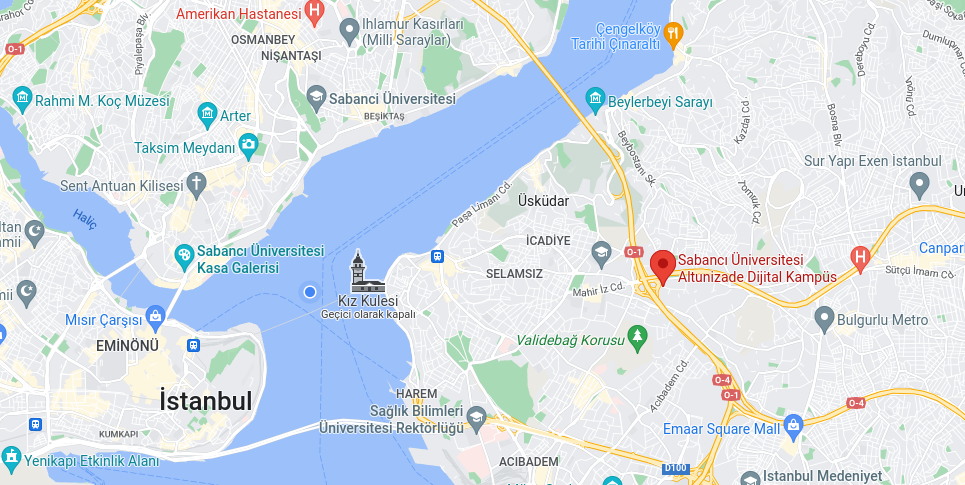
\includegraphics[width=0.7\textwidth]{altunizade_2.png}
\end{figure}


% SPONSORS
%------------------------------------------------------------------
\chapter{Partner Institutions and Sponsors}

\begin{center}
BAŞARIM 2022 konferansı, Türkiye Yüksek Başarımlı Hesaplama Yetkinlik Merkezi tarafından, EuroCC (951732 sayılı hibe sözleşmesi) projesi desteğiyle düzenlenen bir konferanstır. NVIDIA ve Hewlett Packard Enterprise BAŞARIM 2022 konferansının ana sponsorlarıdır. 
\end{center}

\begin{figure}[!h]
\includegraphics[width=0.45\textwidth]{Nvidia-logo.png}

\includegraphics[width=0.55\textwidth]{hpe_pri_grn_pos_rgb.png}
\end{figure}

\vfill


\newpage

% BACK PAGE
%-----------------------------------------------------------------

\pagecolor{myblue}
\thispagestyle{empty}
\mbox{}

\end{document}
